%
\section{Background an Related Work}
\label{sect:bg-rw}
%
In this section, we review a number of background concepts that form the basis for our discussion in this paper. We will illustrate the concepts using a course management (CourseMan) software example.
\subsection{Domain Models in the Annotation-Based Domain Specific Language \dcsl}
\label{sect:bg-dcsl}
%%%%%%%%%%%%%%%%%%%%%%%%%%%%%%%%%%%%%%%%%%%%%%

\abbrv{Annotation-Based Domain Specific Language}{\textbf{aDSL}} is coined in~\cite{nosal_language_2016} as an attempt to formalise the notion of fragmentary, internal DSL~\cite{fowler_domain-specific_2010} for the use of annotation to define DSLs. An aDSL is defined based on an OOPL's abstract syntax model~\cite{le_domain_2018} that consists of the following meta-concepts: class, field, method, parameter, annotation, and property. These meta-concepts are common to two popular host OOPLs: Java~\cite{gosling_java_2014} and C\#~\cite{hejlsberg_c_2010}.

%
We stated in~\cite{le_domain_2018} that using aDSL for DDD brings three important benefits for domain modeling: feasibility, productivity, and understandability. Feasibility comes from the fact the domain model is feasible for implementation in a host OOPL. Productivity is achieved by leveraging the host language platform tools and libraries to process and transform the domain model into other forms suitable for constructing the software. Understandability of the domain model code is enhanced with the introduction of domain-specific annotations.

%Within the scope of this paper and based on the DSL classification in~\cite{kleppe_software_2008}, we differentiate between two types of aDSL: horizontal and vertical aDSLs.
%A \textit{vertical aDSL} targets a bounded real-world (vertical) domain. In contrast, a \textit{horizontal aDSL} (\aka technical aDSL) targets a technical (low-level) domain, whose concepts describe the patterns that often underlie a class of vertical domains that share common features. 
%%Thus, horizontal DSL has a wide scope of application because it is used to build a class of vertical DSLs.
%More specifically, a horizontal aDSL is a DSL internal to a host OOPL, whose domain is a technical one and that uses a set of annotations to model the domain concepts.

%For example, the \courseman's domain model presented in Figure~\ref{fig:arch-model-courseman} can be used as the meta-model for a vertical aDSL for the \courseman~domain. We discussed in~\cite{le_domain_2018} how this domain model is expressed in a horizontal aDSL named \dcsl. A partial \dcsl's domain model of \courseman~is shown in Figure~\ref{fig:dcsl_courseman}. We will review \dcsl~and explain this example in the next subsection.
% In Section~\ref{sect:agl}, we propose another horizontal aDSL for expressing activity graphs. 

\abbrv{Domain class specification language}{\name{DCSL}}~\cite{le_domain_2018} is a horizontal aDSL that we developed to express domain models.
A key feature of \name{DCSL} is that its meta-concepts model the generic domain terms that are composed of the core OOPL meta-concepts and constraints. More specifically, meta-concept \textbf{Domain Class} is composed of meta-concept \clazz{Class} and a constraint captured by an annotation named \clazz{DClass}. This constraint states whether or not the class is mutable. Similarly, meta-concept \textbf{Domain Field} is composed of meta-concept \clazz{Field} with a set of state space constraints. 
These constraints are represented by an annotation named \clazz{DAttr}. 
Meta-concept \textbf{Associative Field} represents Domain Field that realizes one end of an association between two domain classes. \dcsl~supports all three types of association: one-to-one (\abbr one-one), one-to-many (\abbr one-many) and many-to-many (\abbr many-many). 
Finally, meta-concept \textbf{Domain Method} is composed of \clazz{Method} with a commonly-used constraints and behaviour types that are often imposed on instances of these meta-concepts in a domain model. The essential behavior types are represented by an annotation named \clazz{DOpt} and another annotation named \clazz{AttrRef}. The latter references the domain field that is the primary subject of a method's behavior.

Syntactically, we write a \dcsl~model directly using the host OOPL's syntax. For exposition purposes, however, we write this model using an extended UML graphical notation that uses a \textit{structured text box} for writing annotations. Specifically, non-annotation elements are drawn using the usual UML class diagram notation. On the other hand, the annotation elements are drawn using UML note box. Annotation assignment is represented by a dashed grey line, whose target element end is marked with the attachment symbol (\drawFilledRect[gray]{0.15cm}{0.15cm}). The note box content has the form $ A \; \{ props \} $, where $ A $ is the annotation name and $ props $ is a property listing. Each entry specifies the initialization of a property to a value. 
%If this value is another annotation element then this element is written using a nested, borderless note box. 
The entries are separated by either a next line or a comma (`,') character.

Another feature of the above notation is the use of a virtual (dashed) association line to represent a pair of \clazz{DAssoc} elements that help realise the association ends of an association. This association line is more compact and thus helps significantly ease drawing and improves readability of the model. 
We will often use the term ``association'' to refer this association line and the \Name{DCSL} model elements that realise it.

\begin{figure}[ht]
	\centering
	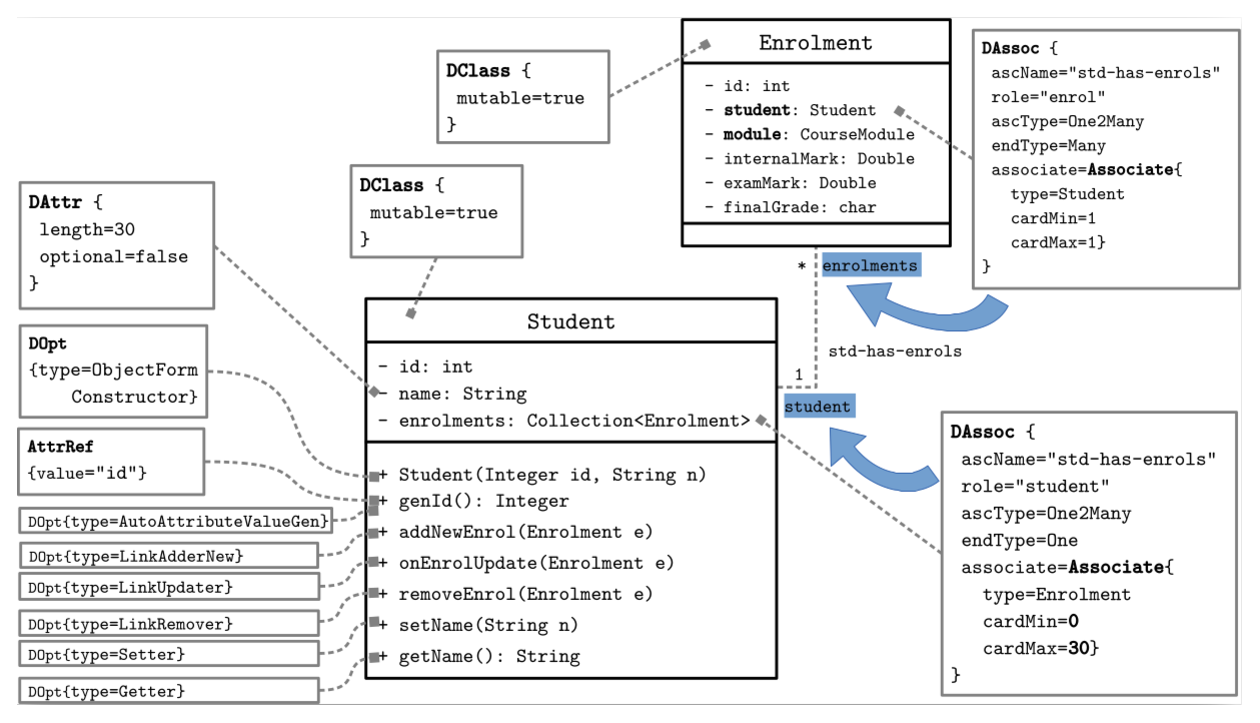
\includegraphics[scale=0.35]{dcsl-model-courseman}
	\caption{A partial \courseman domain model expressed in \dcsl~(adapted from~\cite{le_domain_2018}).}
	\label{fig:dcsl_courseman}
\end{figure}

Figure~\ref{fig:dcsl_courseman} shows a partial \courseman's domain model expressed in \dcsl. This model involves two domain classes: \clazz{Student} and \clazz{Enrolment}. 
%Class \clazz{Enrolment} realises the many-many association between \clazz{Student} and \clazz{Course} (encapsulated by \clazz{CourseModule} as explained in SubSection~\ref{sect:bg-arch}). 
Both of them are assigned with a \clazz{DClass} element, which states that they are mutable domain classes. In particular, class \clazz{Student} has three domain fields: \attribn{id}, \attribn{name}, and \attribn{enrolments}. Domain field \attrib{Student}{name} is illustrated with an \clazz{DAttr} element which states that it is an optional domain field, whose maximum length is 30 (characters). An optional domain field means that the value of this field needs not be initialised when an object is created. Domain field \attrib{Student}{enrolments} is an associative field, which is assigned with a \clazz{DAssoc} element. This element specifies the \clazz{Student}'s end of the association with \clazz{Enrolment}. The opposite end of this association is specified by another \clazz{DAssoc} element that is assigned to the associative field \attrib{Enrolment}{student}. The two thick arrows in the figure map the two \clazz{DAssoc} elements to the two association ends. 
%
The seven methods of class \clazz{Student} listed in the figure are domain methods. Each method is assigned with a \clazz{DOpt} element, which specifies the behavior type. For instance, method \clazz{genId}, whose behavior type is \code{AutoAttributeValueGen}, is additionally assigned with an \clazz{AttrRef} element, which references the name of the domain field \attrib{Student}{id}. This means that \clazz{genId} is the method that automatically generates values for \attrib{Student}{id}.

%%%%%%%%%%%%%%%%%%%%%%%%%%%%%%%%%%%%%%%%%%%%%%
\subsection{The Module-Based Software Architecture MOSA}
\label{sect:bg-arch} %
%%%%%%%%%%%%%%%%%%%%%%%%%%%%%%%%%%%%%%%%%%%%%%

To construct DDD software from the domain model requires an architectural model that conforms to the generic layered architecture~\cite{evans_domain-driven_2004, vernon_implementing_2013}. A key requirement of such model is that they position the domain model at the core layer, isolating it from the user interface and other layers. Evans~\cite{evans_domain-driven_2004} suggests that the MVC architecture model~\cite{krasner_description_1988} is one such model. The existing DDD frameworks~\cite{dan_haywood_apache_2013,paniza_learn_2011} support this suggestion by employing some form of MVC architecture in their designs. We observe from all of these works that the user interface plays an important role in presenting a view of the domain model to the stakeholders in such a way that help them to effectively build the domain model. We thus argue that the MVC architecture must be the backbone of any DDD tool that conforms to the DDD's layered architecture. 

Our previous works~\cite{le_tree-based_2015, le_generative_2018} propose a variant of the MVC architecture for DDD software, called \abbrv{module-based software architecture}{MOSA}. A key feature of this architecture is that it supports the automatic generations of software modules from the domain model and of the software from these modules.
%
A \textbf{MOSA model} consists in a set of MVC-based module classes. 
A \textbf{module class} is an MVC-based structured class~\cite{omg_unified_2015} that represents modules. This class is composed of three components: a domain class (the model), a view class (the view) and a controller class (the controller). The module class becomes the \textit{owner} of the model, view and controller. The view and controller are parameterized classes that are created by binding the template parameters of two library template classes, named \clazz{View} and \clazz{Controller} (\resp), to the domain class.
%
We present in~\cite{le_generative_2018} a technique for semi-automatically generating a module class from the domain class that it owns. Further, the view is designed to reflect the model structure. A set of module classes are used as input for the \jdomainapp~software framework~\cite{le_jdomainapp_2017} to automatically generate software. In this paper, we will assume that a module class is defined for every domain class.

\begin{figure}[ht]
	\centering
	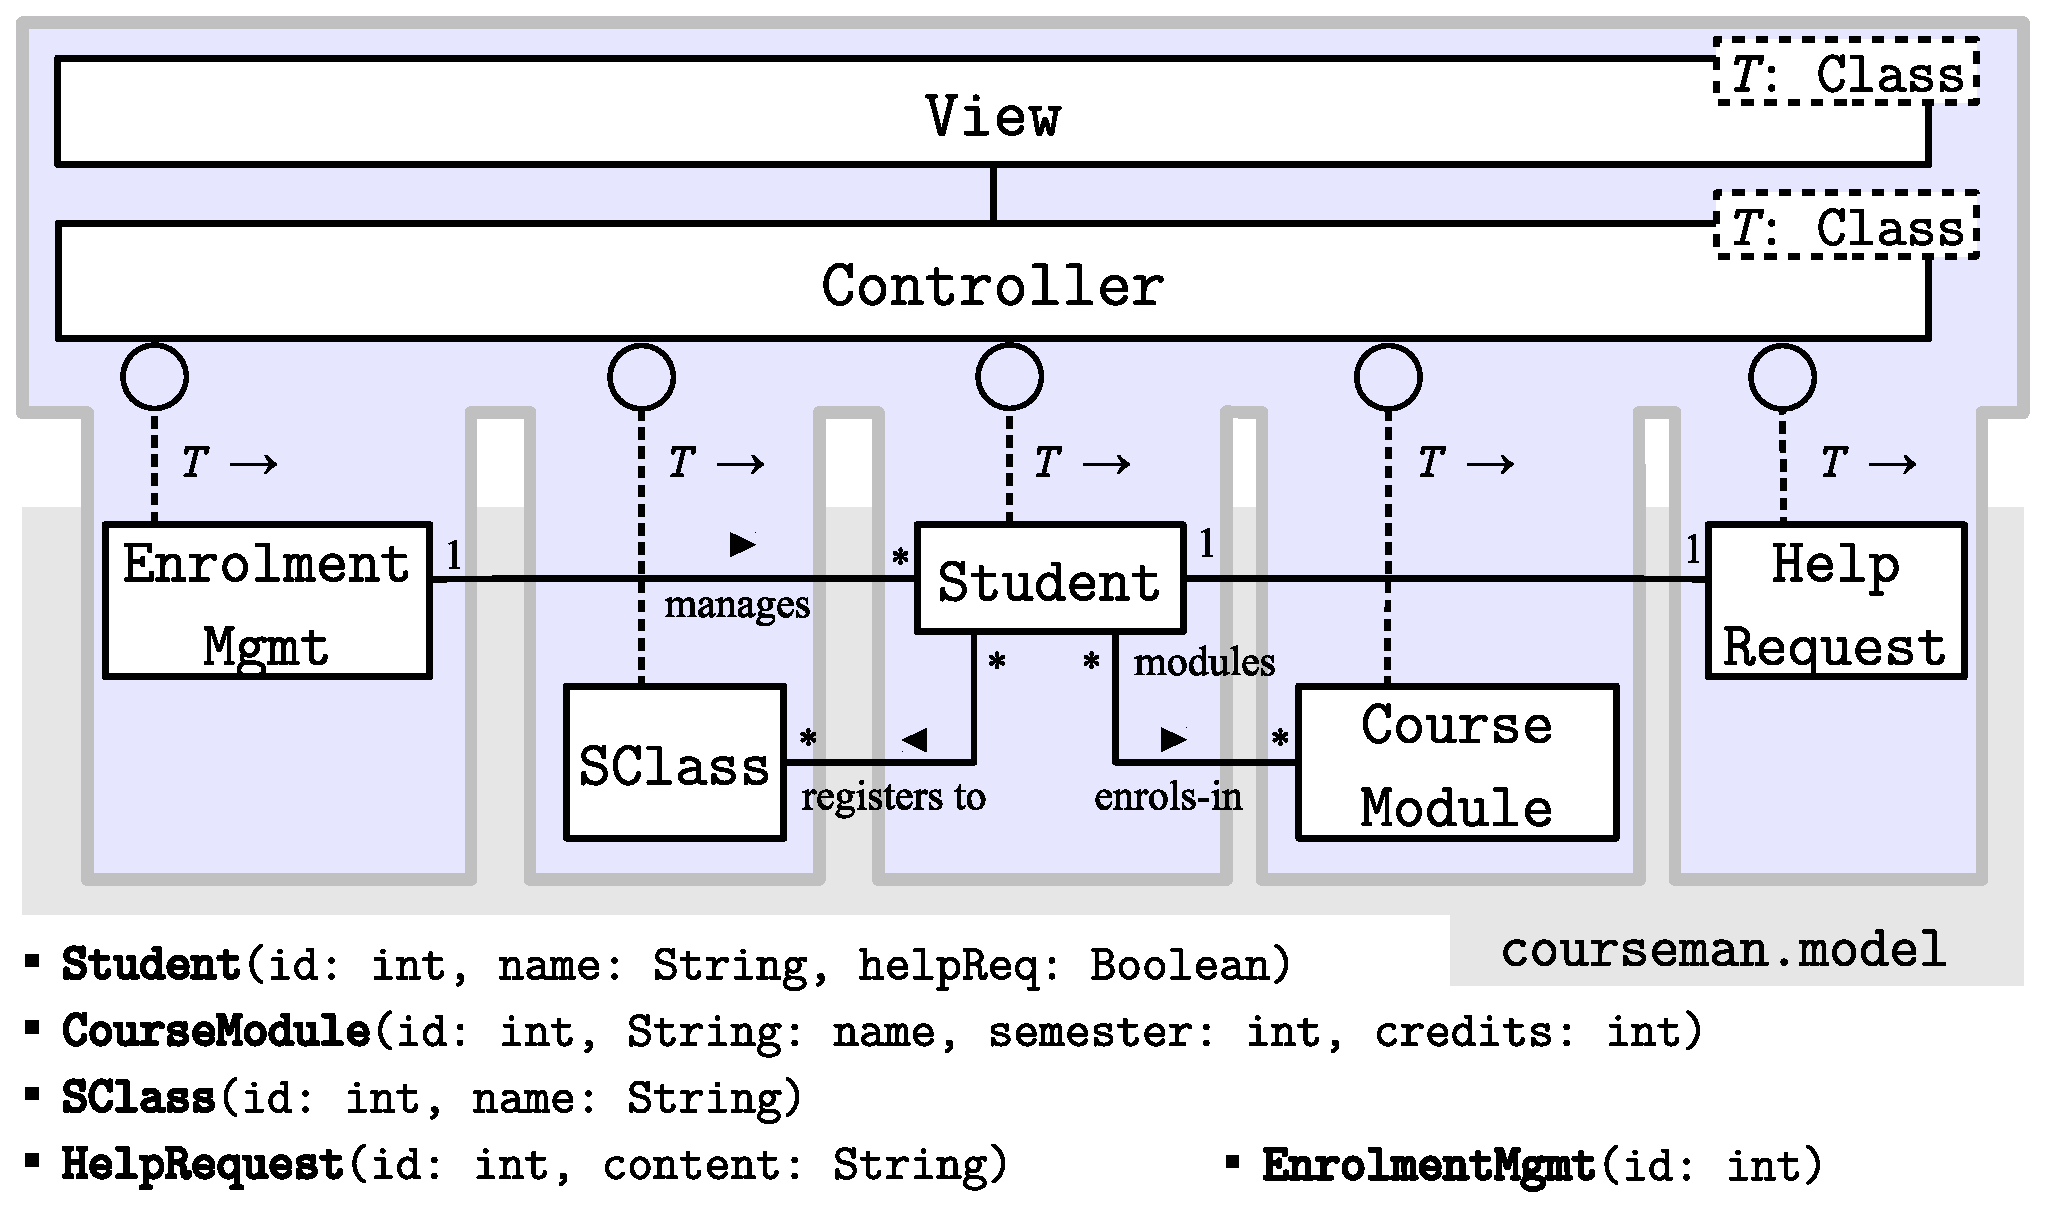
\includegraphics[scale=0.33]{sw-arch/arch-model-courseman}
	\caption{The MOSA model of \courseman.} %
	\label{fig:arch-model-courseman}
\end{figure}

%
To illustrate, the top-half of the MOSA model in Figure~\ref{fig:arch-model-courseman} shows five module classes of \courseman. The parameter bindings are depicted by dashed lines, whose \clazz{Controller}'s and \clazz{View}'s ends are drawn with the symbol `$\bigcirc$'. 
%
%To ease discussion, we name the module classes after their domain classes using the prefix \strq{Module}.
For example, the module class \clazz{ModuleStudent} is composed of three component classes: the domain class is \clazz{Student}, the view is \clazztemplate{View}{\clazz{Student}} and the controller is \clazztemplate{Controller}{\clazz{Student}}.

We argue that MOSA captures the essence of object-oriented software design in a modular, MVC-based design structure. According to Booch~\cite{booch_object-oriented_1986}, an object-oriented software consists of objects and their interactions that are realized though behavior invocation. Given that the domain model is expressed in \dcsl, the MOSA model that has this model at its core helps produce software that possesses the essential behaviors. First, objects are instances of the domain classes in the domain model, which are represented in \dcsl~with the essential structural features. Second, interaction among the objects of a group of domain classes is performed through an event-based message passing mechanism that is managed by the owner modules of these domain classes. This mechanism, which is described in detail in~\cite{le_jdomainapp_2017}, maps events to the essential behaviors that are supported in \dcsl. The events can be triggered by the user interaction on the view of a concerned module. 

However, in~\cite{le_domain_2018} we scoped our use of MOSA at the boundary of the domain model and assumed that this model is connected to the rest of MOSA model via an activity graph. To express this graph in the context of MOSA requires exposing the component interface of the software modules and connecting this interface to the graph. We call this interface the module interface and discuss its design in Section~\ref{sect:actSemantics}. 
%We propose a language for expressing activity graphs in Section~\ref{sect:agl}.
%%%%%%%%%%%%%%%%%%%%
\subsection{Related Work}\label{sect:relatedwork} %
We position our work at the intersection between the following areas: DSL engineering, DDD, MVC architecture, model-driven software engineering (MDSE), and attribute-oriented programming (AtOP).
%, and aspect-oriented software design (AOD).

\textbf{\textit{DSL Engineering.}}
DSLs~\cite{van_deursen_domain-specific_2000, mernik_when_2005} can be classified based on the domain \cite{kleppe_software_2008}, as vertical or horizontal, or based on the relationship with a host language \cite{fowler_domain-specific_2010, van_deursen_domain-specific_2000, mernik_when_2005}, as internal or external. 
%In principle, internal DSL has a closer relationship with the host language than external DSL. A typical internal DSL is developed using either the syntax or the language tools of the host language. 
%In contrast, a typical external DSL has its owns syntax and thus requires a separate compiler to process. 
%
Our proposed \agl~is a type of fragmentary, internal, and horizontal DSL. The shared features that are captured in \agl~are those that form the activity graph domain. To the best of our knowledge, \agl~is the first aDSL that is defined for this purpose.

\textbf{\textit{DDD.}}
The idea of combining DDD and DSL to raise the level of 
abstraction of the target code model has been advocated in~\cite{fowler_domain-specific_2010} by both the DDD's author and others. However, the work in~\cite{fowler_domain-specific_2010} does not discuss any specific solutions.
In this paper, we extended the DDD method~\cite{evans_domain-driven_2004} to construct a unified domain model. We combine this with an activity graph model to operate in a module-based software architecture. The unified model and the activity graph model are expressed in two aDSLs (\dcsl~and \agl, \resp).
%%
%On the other hand, existing DDD frameworks (ApacheIsis~\cite{dan_haywood_apache_2013} and OpenXava~\cite{paniza_learn_2011}) has only a partial support for behavioural modeling through the use of action. They lack support for a behavioural modeling method. Our combination of two aDSLs (\dcsl~and \agl) helps fills this gap. 

\textbf{\textit{Behavioral modeling with UML activity diagram.}}
Although in his book~\cite{evans_domain-driven_2004} Evans does not explicitly mention behavioral modeling as an element of the DDD method, he does consider object behavior as an essential part of the domain model and that UML interaction diagrams would be used to model this behavior. 

%For example, in Chapter 2 of the book, when discussing the use of documents and diagrams (\ie models) in the ubiquitous language, Evans states the followings:
%
%\begin{itemize}
%  \item ``the attributes and relationships are only half the story of an object model. But the behavior of those objects and the constraints on them are not so easily illustrated. Object interaction diagrams can illustrate some tricky hotspots in the design...''
%  
%  \item ``Behavioral responsibilities of an object can be hinted at through operations names, and implicitly
%  demonstrated with object interaction (or sequence) diagrams.''
%%  , but they cannot be stated. So, this falls to supplemental text or conversation. In other words, UML diagrams cannot convey two of the most important aspects of a model: the meaning of concepts it represents, and what they are meant to do.
%\end{itemize}

In UML~\cite{omg_unified_2015} (\S{13.2.1}), interaction diagrams (such as sequence diagrams) are only one of three main diagram types that are used to model the system behavior. The other two types are state machine (\S{14}) and activity diagram (\S{15, 16}). Although in the book, Evans only uses sequence diagrams as an example, in the ApacheIsis framework~\cite{dan_haywood_apache_2013} that directly implements the DDD's philosophy, a simple action language is used to model the object behavior. This language is arguably a specific implementation of the action sub-language (\S{16}) of UML activity diagram. It leverages the annotation construct of OOPL to specify a class operation with a pre-defined behavior type. 
However, ApacheIsIs lacks support for a behavioral modeling method. Our combination of two aDSLs in this paper helps fill this gap.

Our definition of module action in this paper incorporate the notion of state, which is more formally modeled in another UML behavioral modeling language called Behavior State Machines (BSM) (\S{14.2}~\cite{omg_unified_2015}). 
As discussed in~\ref{sect:actSemantics}, our notion of module action's pre- and post-states looks at a similar view with BSM. The difference is that our notation emphasizes the actual behavior, while BSM focuses on the behavior's effects in terms of states and state transitions.

%page break
%\pagebreak
\textbf{\textit{Unified modeling with UML diagrams.}}
There have been works attempting to combine UML structural and behavioral diagrams to construct a system model, similar in spirit to the unified model that we proposed in this paper. Intuitively, this makes sense because the two diagram types address the two core (static and dynamic) aspects of a system. Two works~\cite{kohler_integrating_2000, niaz_object-oriented_2005} discuss combining UML class and state machine diagrams to model the system. Another work~\cite{selonen_transformations_2003} explains the relationships between UML structural and behavioural diagrams and how these relationships can be leveraged to build a complete system model. In particular, this work highlights a strong relationship between state machine (\aka statechart) and activity diagram -- an insight that we also discovered in this paper. 

Our proposed unified domain modeling is novel in that it combines UML class and activity diagrams by incorporating the domain-specific structure (activity class and associations) into the class diagram, thereby creating a unified model. In the spirit of the DDD's layered architecture, we separated the activity graph component of activity diagram from the unified model and created a separate aDSL (\agl) for it. The unified model and activity graph are connected by virtue of the fact that nodes in the graph execute actions of the modules that own the domain classes in the model.

\textbf{\textit{MVC architecture.}}
In practical software development, the MVC (or other equivalent) architecture models are adopted so that the software can have some sort of GUI to assist the development team in constructing it. The main reason for this is rooted in a general understanding (at least up to recently) that software construction can not be fully automated~\cite{fuggetta_software_2014}, due primarily to the human factors that are involved in the development process. 
%
MVC is considered in~\cite{calvary_single-user_1997} to be one of several so-called agent-based design architectures, which help make software developed in them inherently modular and thus easier to maintain. 
Software that is designed in MVC consists of three components: model, view, and controller.
The internal design of each of the three components is maintained independently with minimum impact on the other two components. Modularity can further be enhanced by applying the architecture at the module's level (\eg by adopting another agent-based design architecture named PAC~\cite{coutaz_pac:_1987}), thereby creating a hierarchical design architecture in which a software is composed of a hierarchy of software modules. A software \textit{module} (called PAC object in~\cite{coutaz_pac:_1987} and, more generally, agent in~\cite{calvary_single-user_1997}) is a realization of a coherent subset of the software's functions in terms of the architectural components.

%Conceptually, the model component of a software is the domain model. It includes a set of domain classes that capture data about the entities of interest in the application domain. The view component of a software is a set of user interface (UI) classes that are used to capture data about the domain objects. Each class presents to the user a coherent view of a domain class and to make it easy for her to interact with this view.
%

Our method is novel in the treatment of MVC. We basically use it at the `micro' level to design each software module as a self-contained MVC component. We then expose a module interface and combine it with the activity graph design.

\textbf{\textit{MDSE.}}
The idea of combining MDSE with DSLs is formulated in \cite{kleppe_software_2008, brambilla_model-driven_2012}. This involves applying the meta-modeling process to create meta-models of software modeling languages (include both general-purpose languages and DSLs). 
Our \agl's specification follows the pattern-based meta-modeling approach, but targets internal DSL.

%\subsubsection*{DSLs for Software modeling}
Our method is similar to the method proposed in \cite{warmer_model_2007, warmer_building_2006} in the use of a combination of DSLs to build a complete software model. 
%In these work, a 3-step method is outlined, which includes: (1) determine the software architecture, (2) develop DSLs that fit this architecture and (3) combine the DSLs by defining transformations between them. 
%
However, our method differs in two technical aspects. 
%First, our work is applicable to a more general class of architectures, which is characterised by a set of modules that interact via events. 
%The scope of a module is comparable to that of partial model. 
%Our module-based software architecture is a general architecture style, for which service-oriented architecture is a specialisation. 
First, we use (internal) aDSLs as opposed to external DSLs. Second, our method (being a DDD type) clearly highlights the boundary of the domain model and, based on this, proposes to use only two aDSLs. The above works use four DSLs and do not clearly indicate which ones are used for constructing the domain model and which are used to build other parts of the software model. 
%Our DSLs are more technical (more generic) than the above work. Specifically, \dcsl~realises the patterns that underlie both the data contract and business class DSLs. \agl, which is defined based on the UML activity diagram sublanguage, realises the patterns that underlie both web scenario and service DSLs.

\textbf{\textit{AtOP.}}
Our idea of using annotation to represent modeling rules and constraints is inspired by AtOP \cite{wada_modeling_2005, cepa_representing_2005,sulir_recording_2016,balz_embedding_2012}. In principle, AtOP extends a conventional program with a set of attributes, which capture application- or domain-specific semantics \cite{cepa_representing_2005}. These attributes are represented in contemporary OOPLs as annotations. 
%As discussed above, the existing DDD frameworks also adopt this representation.

%\subsubsection*{Using AtOP for MDSE}
With regards to the use of AtOP in MDSE, a classic model of this combination is used in the development of a model-driven development framework, called mTurnpike \cite{wada_modeling_2005}. 
%This framework combines AtOP with model-driven development in a top-down fashion, with an aim to define domain-specific concepts at both the modeling and programming levels. 
%
More recently, the work in \cite{balz_embedding_2012} proposes a bottom-up MDSE approach, which entails a formalism and a general method for defining annotation-based embedded models. 
%
Our method differs from both \cite{wada_modeling_2005,balz_embedding_2012} in two important ways: 
%the support for both structural and behavioural modeling 
(1) the combination of two aDSLs that can be used to express the configured unified model, and (2) how this model is used to automatically generate the entire software. 